\documentclass{article}
\usepackage{spikey}
\usepackage{amsmath}
\usepackage{mathrsfs}
\usepackage{amssymb}
\usepackage{soul}
\usepackage{float}
\usepackage{graphicx}
\usepackage{hyperref}
\usepackage{fancyhdr}
\usepackage{xcolor}
\usepackage{chngcntr}
\usepackage{centernot}
\usepackage[shortlabels]{enumitem}
\usepackage[margin=1truein]{geometry}
\usepackage{tkz-graph}
\usepackage{dsfont}
\usepackage{caption}
\usepackage{subcaption}

\usepackage{setspace}
\linespread{1.15}
\usepackage[margin=1truein]{geometry}

\counterwithin{equation}{section}
\counterwithin{figure}{section}

\pagestyle{fancy}
\lhead{Topics in Economics of Information}

\usepackage[
    type={CC},
    modifier={by-nc},
    version={4.0},
]{doclicense}

\title{CSC412/2506 Winter 2020: Probabilistic Learning and Reasoning}
\date{\today}
\author{Tianyu Du}
\begin{document}
    \maketitle
    \tableofcontents
    \newpage
    \section{Introduction}
    
    \section{Probabilistic Models}
	
	\section{Directed Graphical Models}
	\subsection{Decision Theory}
	
	\section{Exact Inference}
	\begin{notation}
		Let $X$ denote the set of all random variables in the model, and
		\begin{enumerate}
			\item $X_{E}=$ The observed evidence;
			\item $X_{F}=$ The unobserved variable we want to infer;
			\item $X_{R}=X-\left\{X_{F}, X_{E}\right\}=$ Remaining variables, extraneous to query.
		\end{enumerate}
		The model defines the joint distribution of all random variables:
		\begin{align}
			p(X_E, X_F, X_R)
		\end{align}
	\end{notation}
	
	\begin{definition}
		The joint distribution over evidence and subject of inference is
		\begin{align}
			p\left(X_{F}, X_{E}\right)=\sum_{X_{R}} p\left(X_{F}, X_{E}, X_{R}\right)
		\end{align}
	\end{definition}
	
	\begin{definition}
		The conditional probability distribution for inference given evidence is
		\begin{align}
			p\left(X_{F} | X_{E}\right)=\frac{p\left(X_{F}, X_{E}\right)}{p\left(X_{E}\right)}=\frac{p\left(X_{F}, X_{E}\right)}{\sum_{X_{F}} p\left(X_{F}, X_{E}\right)}
		\end{align}
	\end{definition}
	
	\begin{definition}
		The distribution of evidence can be computed as
		\begin{align}
			p\left(X_{E}\right)=\sum_{X_{F}, X_{R}} p\left(X_{F}, X_{E}, X_{R}\right)
		\end{align}
	\end{definition}
	
	\subsection{Variable Elimination}
	
	\subsection{Intermediate Factors}
	\begin{figure}[H]
		\centering
		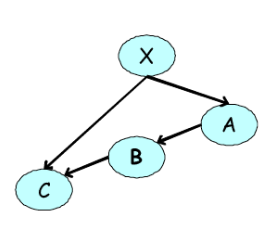
\includegraphics[width=0.3\linewidth]{figures/week_4_2.png}
	\end{figure}
	\begin{align}
		p(A, B, C) &=\sum_{X} p(X) p(A | X) p(B | A) p(C | B, X) \\
		&=p(B | A) \underbrace{\sum_{X} p(X) p(A | X) p(C | B, X)}_{\tx{unnormalized}}
	\end{align}
	\begin{definition}
		A \textbf{factor} $\phi$ describes the local relation between random variables, meanwhile, $\int d\phi$ is \ul{not} necessarily one.
	\end{definition}

	\begin{remark}
		Let $X_\ell \subseteq X$ be a group of local random variables, then $p(X_\ell)$ is automatically a factor $\phi(X_\ell)$.
	\end{remark}

	\begin{align}
		p(A, B, C) &=\sum_{X} \underbrace{p(X) p(A | X) p(B | A) p(C | B, X)}_{\tx{from graphical representation}} \\
		&=\sum_{X} \underbrace{\phi(X) \phi(A, X) \phi(A, B) \phi(X, B, C)}_{\tx{factor representation}} \\
		&=\phi(A, B) \sum_{X} \phi(X) \phi(A, X) \phi(X, B, C) \\
		&=\phi(A, B) \underbrace{\tau(A, B, C)}_{\tx{another factor}}
	\end{align}
	
	\subsection{Sum-Product Inference}
	\begin{theorem}
		Consider a graphical model with random variables $X = Y \cup Z$.
		For an random variable $Y$ in a \ul{directed} or \ul{undirected} model, $P(Y)$ can be computed using the \textbf{sum-product}
		\begin{align}
			\tau(Y) = \sum_z \prod_{\phi \in \Phi} \phi({Scope[\phi]\cap Z}, {Scope[\phi] \cap Y})
		\end{align}
		where $\Phi$ is a set of factors.
	\end{theorem}
	
	\begin{remark}
		For \ul{directed models},
		\begin{align}
			\Phi=\left\{\phi_{x_{i}}\right\}_{i=1}^{N}=\left\{p\left(x_{i} | \text { parents }\left(x_{i}\right)\right)\right\}_{i=1}^{N}
		\end{align}
	\end{remark}
	
%	\begin{example}
%		\begin{figure}[H]
%			\centering
%			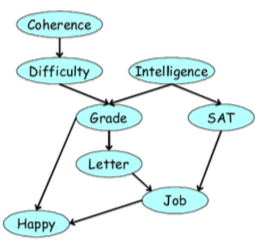
\includegraphics[width=0.3\linewidth]{figures/week_4_3.png}
%		\end{figure}
%		\begin{align}
%			p(C, D, I, G, S, L, H, J)=p(C) p(D | C) p(I) p(G | D, I) p(L | G) P(S | I) p(J | S, L) p(H | J, G)
%		\end{align}
%		using factor representation:
%		\begin{align}
%			\Phi=\{\phi(C), \phi(C, D), \phi(I), \phi(G, D, I), \phi(L, G), \phi(S, I), \phi(J, S, L), \phi(H, J, G)\}
%		\end{align}
%	\end{example}
	
	\subsection{Complexity of Variable Elimination Ordering}
	\begin{theorem}
		The complexity of the variable elimination algorithm is
		\begin{align}
			\mc{O}(m k^{N_{max}})
		\end{align}
		where
		\begin{enumerate}[(i)]
			\item $m$ is the number of initial factors $|\Phi|$;
			\item $k$ is the number of states each random variable takes, assumed to be equal;
			\item $N_i$ is the number of random variables within each summation;
			\item $N_{max} = \max_i N_i$.
		\end{enumerate}
	\end{theorem}
	
	\section{Message passing, Hidden Markov Models, and Sampling}

	\subsection{Message Passing (Computing All Marginals)}
	
	\begin{notation}
		Let $T$ denote the set of edges in a tree. For a node $i$, let $N(i)$ denote the set of its neighbours.
	\end{notation}
	
	The factor of all random variables can be computed following
	
	\begin{align}
		P\left(X_{1: n}\right)
		=\frac{1}{Z} \underbrace{\left[ \prod_{i=1}^n \phi\left(x_{i}\right)
		\right]}_\tx{prior factors}
		\underbrace{\prod_{(i, j) \in T} \phi_{i, j}\left(x_{i}, x_{j}\right)}_\tx{local factors}
	\end{align}
	
	\begin{definition}
		The \textbf{message} sent from variable $j$ to $i \in N(j)$ is
		\begin{align}
			m_{j \rightarrow i}\left(x_{i}\right)
			=\sum_{x_{j}}
			\left [
			\phi_{j}\left(x_{j}\right) \phi_{i j}\left(x_{i}, x_{j}\right)
			\prod_{k \in N(j) \neq i} m_{k \rightarrow j}\left(x_{j}\right)
			\right ]
		\end{align}
	\end{definition}
	
	\begin{algorithm}[Belief Propagation Algorithm]
		Given a tree, inference on an arbitrary node $p(x_i)$ can be computed following:
		\begin{enumerate}
			\item Choose root $r$ arbitrarily;
			\item Pass messages from leaves to $r$;
			\item Pass messages from $r$ to leaves;
			\item Compute inference
			\begin{align}
				p\left(x_{i}\right) \propto \phi_{i}\left(x_{i}\right) \prod_{j \in N(i)} m_{j \rightarrow i}\left(x_{i}\right)
			\end{align}
		\end{enumerate}
	\end{algorithm}
	
	\subsection{Markov Chains}
	\par Using chain rule of probability:
	\begin{align}
		p\left(x_{1: T}\right)=\prod_{t=1}^{T} p\left(x_{t} | x_{t-1}, \ldots, x_{1}\right)
	\end{align}
	
	\begin{definition}
		A Markov chain is said to be \textbf{first-order} if 
		\begin{align}
			p\left(x_{t} | x_{1: t-1}\right)=p\left(x_{t} | x_{t-1}\right)
		\end{align}
	\end{definition}
	
	\paragraph{Simplification} Therefore, for all first-order Markov chains, the full joint distribution can be reduced to
	\begin{align}
		p\left(x_{1: T}\right)=\prod_{t=1}^{T} p\left(x_{t} | x_{t-1}\right)
	\end{align}
	
	\begin{definition}
		A Markov chain is at $m$-order if
		\begin{align}
			p\left(x_{t} | x_{1: t-1}\right)=p\left(x_{t} | x_{t-m: t-1}\right)
		\end{align}
	\end{definition}
	
	\begin{definition}
		A Markov chain is said to be \textbf{homogenous} (i.e., stationary) if
		\begin{align}
			p\left(x_{t} | x_{t-1}\right)=p\left(x_{t+k} | x_{t-1+k}\right) \quad \forall t, k
		\end{align}
	\end{definition}
	
	\paragraph{Parameterization} Assume the random variable $X_t$ takes $k$ states, further suppose the chain is time homogenous. Then characterizing the transition probability
	\begin{align}
		p(x_t | x_{t-1}, x_{t-2}, \cdots, x_{t-m})
	\end{align}
	requires $(k-1) k^m$ parameters.
	
	\subsection{Hidden Markov Models}
		\begin{figure}[H]
		\centering
		\begin{tikzpicture}
		\tikzset{vertex/.style = {shape=circle,draw,minimum size=1.5em}}
		\tikzset{edge/.style = {->,> = latex'}}
		% vertices
		\node[vertex] (x1) at  (0,0) {$x_1$};
		\node[vertex] (z1) at  (0,2) {$z_1$};
		
		\node[vertex] (x2) at  (3,0) {$x_2$};
		\node[vertex] (z2) at  (3,2) {$z_2$};

		\node[vertex] (x3) at  (6,0) {$x_3$};
		\node[vertex] (z3) at  (6,2) {$z_3$};
		
		\node[vertex] (z4) at  (9,2) {$z_{t \geq 4}$};
		%edges
		% Iter 1
		\draw[edge] (z1) to (x1);
		\draw[edge] (z1) to (z2);
		\draw[edge] (z2) to (x2);
		\draw[edge] (z2) to (z3);
		\draw[edge] (z3) to (x3);
		\draw[edge] (z3) to (z4);
		\end{tikzpicture}
		\caption{Hidden Markov Model}
	\end{figure}
	
	\paragraph{Parameterization} Assuming the HMM is \ul{homogenous}, then the set of parameters $\Phi$ consists of
	\begin{enumerate}[(i)]
		\item 
	\end{enumerate}
	
%	\section{Sampling and Monte Carlo Methods}
\end{document}




















